\documentclass[11pt,letterpaper]{article}

\usepackage{pgfgantt}
\usepackage[letterpaper,margin=0.75in,nohead]{geometry}
\usepackage{graphicx}
\usepackage{subcaption}
\usepackage[colorlinks]{hyperref}
\usepackage{url}
\usepackage{breakurl}

\hypersetup{
    colorlinks,
    linkcolor={red},
    citecolor={red},
    urlcolor={blue}
}

% add packages as needed


\title{CIS 6930: Trustworthy Machine Learning\\
	\Large Project Proposal: Title of the Project} %% TODO: replace with the title of your project

%% TODO: your name and email go here (all members of the group)
%% Comment out as needed and designate a point of contact
\author{
        Tanvi Jain \\{\em (Point of Contact)} \\
        tjain@ufl.edu\\
        \and
        Nimish Bajaj \\
        nimishbajaj@ufl.edu\\
}

% set the date to today
\date{\today}


\begin{document} % start document tag

\maketitle


%%% Remember: writing counts! (try to be clear and concise.)
%%% the whole proposal should be about 2 pages (in 11pt font)


%% TODO: write your introduction
%% Must address:
%% - What is the problem?
%% - Why is the problem interested and worth solving?
%% - What are you proposing to do (at high level)?
%%
\section{Introduction}

% TODO:

Determine whether explainable / interpretable ML techniques like LIME and others can provide useful insights into the cause of the unfairness.

A model's accuracy is not always enough to state weather it will perform well in the wild because the accuracy highly depends the data that was used to train and test the model. 
Explaining the results of a model, and identifying what lead to a particular classification can help provide insights into the model.
Once you add interpretability to the model, its result can be easily understood by a domain expert can be verified for correctness. This greatly enhances the trustworthyness of the model.


We are proposing to build a text classification model and explaining the results using LIME, and validate if LIME is able to provide stable and meaningful features. 

%% TODO: write your background and related work
%% Must contain:
%% - Background to make the proposal self-contained
%% - Short related work survey (what are the 3-4 most related papers about? what do they do?)
%% - Why is your proposal novel? What are you proposing to do different?
%%
\section{Background and Related Work}





Since the data contains technical words which are sometimes outside of the english vocabulary, we are going to tune word embeddings for the problem domain.



% TODO:
Write here.

You can cite related publications like so~\cite{vapnik1994measuring} and non-publications (e.g., websites) like so\footnote{Google scholar: \url{https://scholar.google.com}}.


%% TODO: write your proposed approach and describe your plan
%%
%% - Describe your approach to solve the problem
%% - What's your plan?
%% - Be concrete!!
%% 		-- What dataset will you use?
%% 		-- What equipment do you need? How will you get it?
%% 		-- What are you going to measure? What metrics will you use?
%%		-- How will you know whether what you are doing is working?
%% 
\section{Proposed Approach \& Plan}

% TODO:


%% TODO: Write a short timeline of your project
%%
%% - Describe steps and milestones for you project
%% - Briefly state what you hope the final outcome will be. (Will you have preliminary results to include on the presentation/poster?)
%%
%%
%% Keep in mind the project milestones must include mid semester report
%%

Following is the approach we are going to take:


1. Fetch data and take samples as per the distribution of data for train, test and validation

2. Clean and vectorize the data for Neural Network (NN) approach

3. Build a NN architecture to learn classification labels

4. Train, test and validate the neural network

5. Use LIME for model inferencing

6. Manually validate LIME output

\begin{figure}[h!]
	\centering
	\begin{subfigure}[b]{0.4\linewidth}
		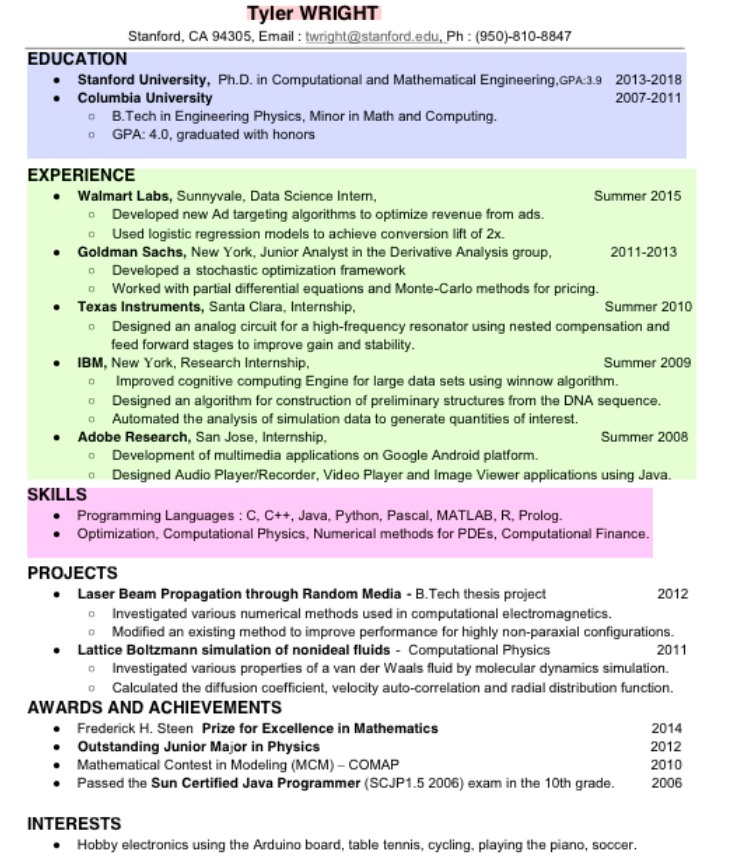
\includegraphics[width=\linewidth]{images/resume.png}
		\caption{Example Input}
	\end{subfigure}
	\begin{subfigure}[b]{0.4\linewidth}
		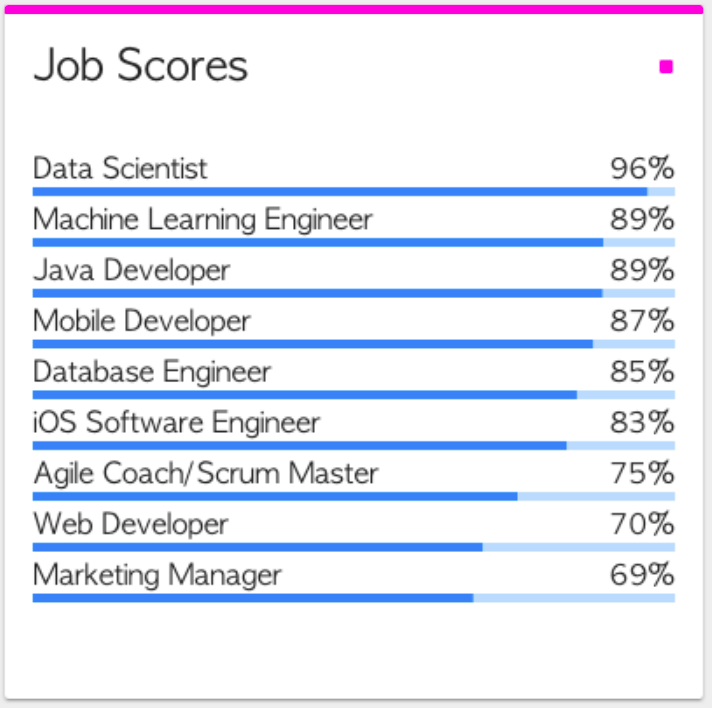
\includegraphics[width=\linewidth]{images/job_title.png}
		\caption{Model prediction}
	\end{subfigure}
	\caption{Model output description}
	\label{fig:coffee}
\end{figure}


\section{Timeline}

% TODO:
\begin{figure}
	
	
	\begin{center}
		
		\begin{ganttchart}[y unit title=0.4cm,
			y unit chart=0.5cm,
			vgrid,hgrid, 
			title label anchor/.style={below=-1.6ex},
			title left shift=.05,
			title right shift=-.05,
			title height=1,
			progress label text={},
			bar height=0.7,
			group right shift=0,
			group top shift=.6,
			group height=.3]{1}{30}
			%labels
			\gantttitle{September 27 - December 7}{30} \\
			\gantttitle{Week1}{3} 
			\gantttitle{Week2}{3} 
			\gantttitle{Week3}{3} 
			\gantttitle{Week4}{3} 
			\gantttitle{Week5}{3} 
			\gantttitle{Week6}{3} 
			\gantttitle{\color{red}Mid Sem}{3}
			\gantttitle{Week8}{3} 
			\gantttitle{Week9}{3} 
			\gantttitle{Week10}{3} \\
			%tasks
			\ganttbar{Research}{1}{6} \\
			\ganttbar{Data sampling}{4}{7} \\
			\ganttbar{Data preprocessing}{6}{12} \\
			\ganttbar{NN architecture}{10}{15} \\
			\ganttbar[]{Model training}{15}{22} \\
			\ganttbar{Model inferencing}{22}{26} \\
			\ganttbar{LIME validation}{24}{28} \\
			\ganttbar[]{Output generation}{27}{30}
			
		\end{ganttchart}
	\end{center}
	\caption{Gantt Chart}
\end{figure}

%%%%

\bibliography{refs}
\bibliographystyle{plain}


\end{document} % end tag of the document